A Soft Error or Single Event Upset is a random, non-catastrophic error, where radiation causes
a perturbation to a circuit by temporarily altering a single signal or datum.
Detecting and mitigating such errors is highly important in some fields, such as satellite design, 
where high design costs, harsh environments, and difficulties to repair once deployed make it necessary. 
However with the continuing increasing of semiconductor densities the current soft error
challenges experienced in space will likely be future problems for terrestrial devices\cite{normand1996single}\cite{henkel2013reliable}.

FPGA devices work through mapping circuit descriptions into a collection of Logic Blocks,
which are described in programmable look-up-tables and routed together via
programmable switchboxes.
Configuration data for both the look-up-tables and switchboxes are stored in a
configuration memory, which means soft errors can either change the functionality
of Logic Blocks or can change the routing between them.
Other memories called Block memory and flip-flops are also present in FPGA devices,
and soft errors in these regions can alter the state of the circuit but not the
circuits functionality.

%How this changes the protection strategy compared to software and VLSI
For VLSI/ASIC designs registers are the most vulnerable to soft-errors, with
combinational logic contributing very little \cite{baumann2005soft} this makes
approaches which asses and protect vulnerable registers promising \cite{chen2014reliability}.
However in FPGA devices the most vulnerable region is the configuration memory
so such approaches would have little impact requiring alternative methods.

%ECC and frame based checking approaches
Circuits described within configuration memory are usually protected in one of two ways,
either the circuit is replicated with comparison, or ECC/CRC signals associated with
frames of the configuration memory are scanned for errors.
Replication uses extra area and power however error detection latency is low,
while ECC/CRC checks consume less area and power but detection latency is higher and
it is limited to only protecting configuration memory.

\begin{figure}[h]
\centering
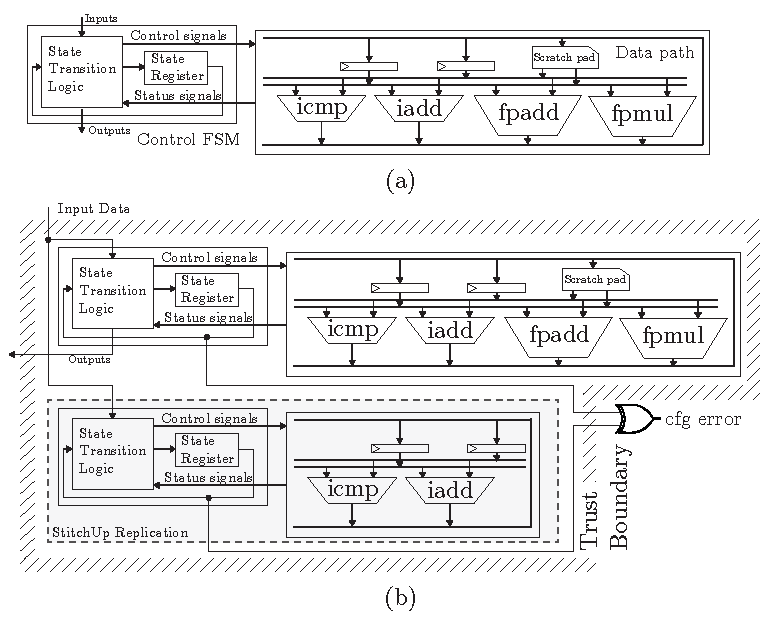
\includegraphics[width=3.5in]{./imgs/StitchUpReplication.pdf}
\caption{StitchUp Replication for the Matrix Multiplication example, with Trust Boundary}
\label{fig:HLSArch}
\end{figure}

For this paper our \emph{fault model} assumes that a single soft error
can occur at most every clock cycle, and that this error can effect block memory,
configuration memory, or flip-flops.
Since errors are not solely within the configuration memory replication must be used
instead of ECC/CRC codes to fully protect our control structure.
Figure \ref{fig:HLSArch} shows a StitchUp generated circuit for the matrix multiplication
example in Listing \ref{lst:MMM}, with the original circuit on top and the
control-flow structure shadow beneath it.
StitchUp aims to protect all configuration, block, and Flip-flop bits within the
trust boundary (grey box) as everything outside, such as routing to
external I/O or DDR, is not protected.

